\section{Kapacitetudnyttelse}
Kapacitetsudnyttelse anvendes for at analysere OA's ressourcer ift. patientbyrden. Forholdet mellem aktivitet og kapacitet betegner kapacitetsudnyttelsen, hvilket ses af \figref{kapacitet}. Aktivitet omhandler patient og kontakt, herunder består kontakt af forundersøgelse, behandling og kontrol af patienter. Kapacitet omfatter antallet af personale, udstyr og rum, hvor personalet består af læger, sygeplejersker og sekretærer. Udstyret beskriver antallet af maskiner på en afdeling, og antallet af rum beskriver opbevarelsen af udstyret. Den samlede kapacitetsudnyttelse er defineret ud fra, at der produceres mest muligt for de investerede ressourcer.\cite{Company2013} 

\begin{figure}[H]
	\flushleft 
	\centering
	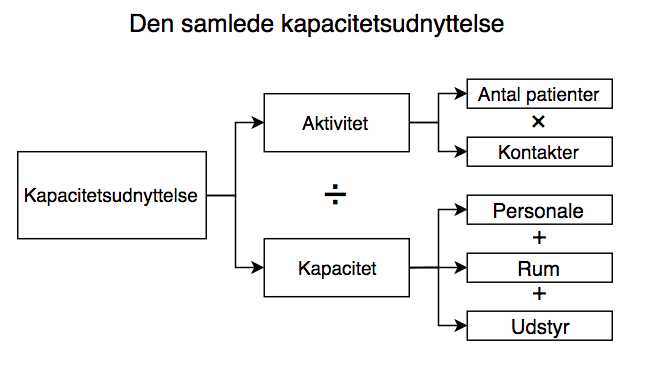
\includegraphics[scale=.5]{figures/Kapacitetsudnyttelse.png}
	\flushleft
	\caption{\textit{Den samlede kapacitetsudnyttelse, som er definineret ved forholdet mellem aktivitet og kapacitet. Aktivitet omfatter antallet af patienter samt kontakter, og kapacitet omfatter personale, rum og udstyr.}\cite{Company2013}}
	\label{kapacitet}
\end{figure}

\noindent
Et andet begreb er belægning, som er defineret ud fra antallet af patienter, der er normeret til på en afdeling\cite{Heidmann2014}. Når en $100~\%$ belægning opnås, svarer dette til, at alle disponible sengepladser på en afdeling er taget i brug. Ved en belægning på over $100~\%$ betyder det, at der er flere patienter end afdelingen er normeret til, hvilket vil sige, at afdelingen yder mere end der er kapacitet til. Ud fra \figref{kapacitet} vil dette betyde, at der ikke er ligevægt mellem aktivitet og kapacitet, hvilket i dette tilfælde vil forårsage kapacitetsmangel på afdelingen. 


\subsection{Belægningsgrad på ortopædkirurgisk afdeling}\label{omfang}
Der ønskes en fuld kapacitetsudnyttelse på OA for at udnytte ressourcerne på afdelingen, hvorfor alle sengepladser ønskes at være i brug. Antallet af de anvendte disponible sengepladser beskriver belægningsgraden. På OA opleves en varierende belægningsgrad. På \figref{maxminbelaeg} ses belægningsgraden fra år $2014$ til $2016$ på OA.\cite{SDS2015}

\begin{figure}[H]
	\flushleft 
	\centering
	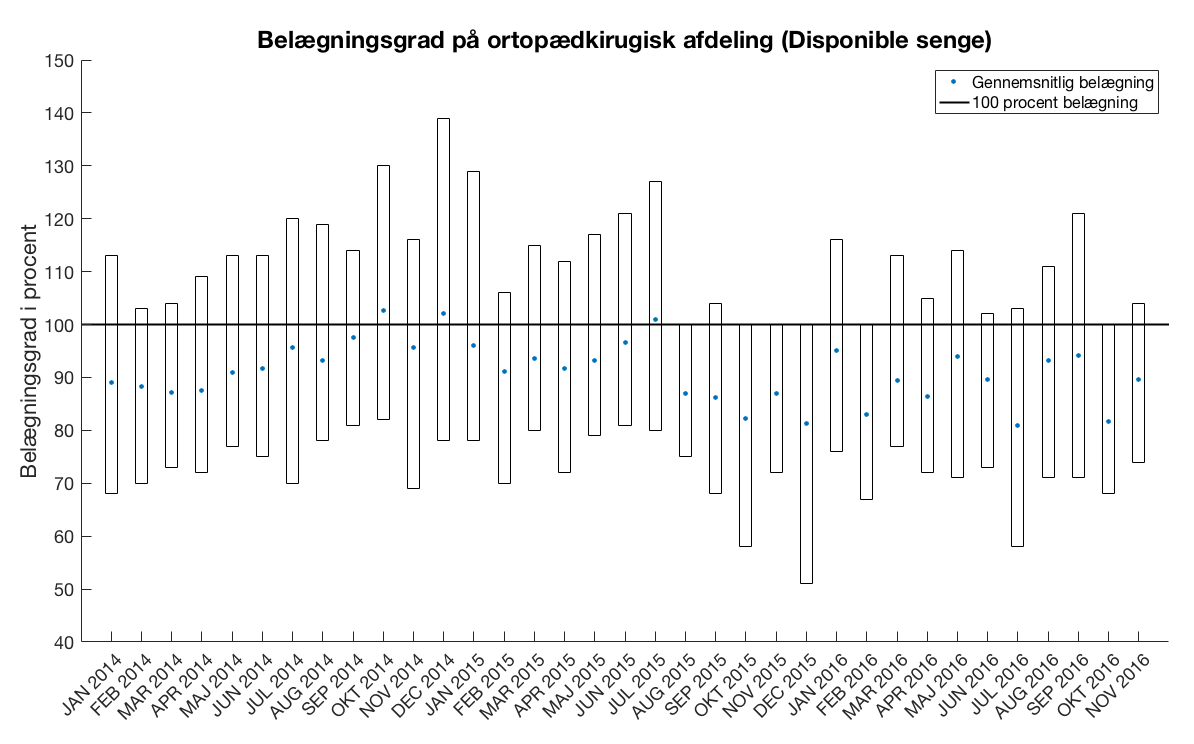
\includegraphics[scale=.45]{figures/belaegningsgradny.png}
	\flushleft
	\caption{\textit{Belægningsgraden på OA målt over $35$ måneder fra år $2014$ til $2016$. Søjlerne viser belægning ift. $100~\%$, hvortil maksimal og minimal belægning ligeledes illustreres. De blå punkter viser den gennemsnitlige belægning for hver måned.}\cite{SDS2015}}
	\label{maxminbelaeg}
\end{figure}

\noindent
Det fremgår af \figref{maxminbelaeg}, at OA oplever en belægning hhv. over og under den ønskede belægning på $100~\%$. Den maksimale belægning fremkommer i december måned år 2014 og er på $139~\%$. Maksimal belægning kan indikere, at der er flere indlagte patienter end afdelingen er disponeret til, herved har afdelingen oplevet kapacitetsmangel. Den minimale belægning forekommer i december måned år 2015 og er på $51~\%$. Dette kan indikere, at der ikke har været et tilstrækkeligt antal patienter, hvilket ligeledes medfører ubalance i kapacitetsudnyttelsen. Af \figref{maxminbelaeg} er den gennemsnitlige belægning pr. måned hyppigst under $100~\%$. I oktober samt december måned år $2014$ og juli år 2015 opleves dog en gennemsnitlig belægning over $100~\%$. Den gennemsnitlige belægning ses varierende mellem $80$ og $100~\%$ for de resterende måneder, hvilket kan indikere, at afdelingen oplever kapacitetsmangel i kortvarige perioder.
Det fremgår ikke af den anvendte data, hvorvidt belægningen over $100~\%$ opleves i timer eller flere døgn.
For at underbygge belægningsgraden yderligere, illustrerer \figref{andeldage} andel af dage med en belægningsgrad over $100~\%$ pr. måned. 
Denne graf er udarbejdet ud fra OA over de samme 35 måneder som \figref{maxminbelaeg}.\cite{SDS2015} 

\begin{figure}[H]
	\flushleft 
	\centering
	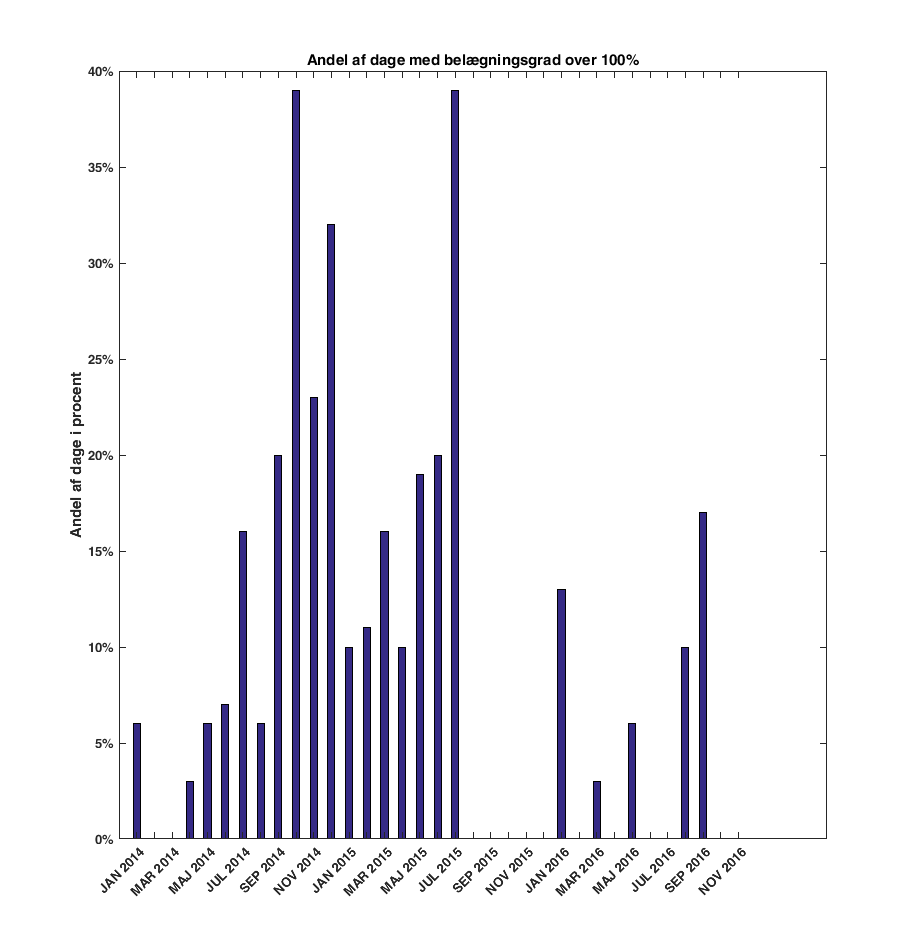
\includegraphics[scale=.4]{figures/andelAfDage.png}
	\flushleft
	\caption{\textit{Andel af dage med en belægning over $100~\%$ for OA målt over $35$ måneder fra år $2014$ til $2016$.}\cite{SDS2015}}
	\label{andeldage}
\end{figure}

\noindent
Det fremgår af \figref{andeldage}, at der i oktober måned år $2014$ samt juli måned år 2015 ses en belægning på over $100~\%$ i $39\%$ af måneden. Sammenlignes der med \figref{maxminbelaeg} ses der i oktober måned år 2014 en belægning på $130~\%$. I juli måned år 2015, der ligeledes havde en belægning over $100\%$ i $39\%$ af måneden, ses en belægning på $127\%$. 
Ud fra det anvendte data fremgår det ikke, hvor mange patienter, der udgør en belægningsgrad over $100~\%$, samt hvor længe de enkelte patienter er indlagt på afdelingen. Da belægningsgraden og andel af dage med belægningsgrad over $100~\%$ kan variere for hver måned, anses $35$ måneder ikke som værende repræsentativ for at kunne vurdere problemets omfang. Ud fra belægningsgraden kan det dog tyde på, at en effektivisering af planlægningen af patienter på OA vil kunne medføre en balance i kapacitetsudnyttelsen.
